\chapter{Installation Guide}
\label{chap:appendix-d}
This guide will outline the requirements and installation procedure to get the automation platform up and running. The guide will assume that the user has a basic understanding of Linux and the command line as well as Cisco ACI and VMware vCenter.

This solution is designed to allow a testing environment to provide OOB connectivity to a variety of projects within a testing environment through the use of a web UI. It achieves this through the use of Cisco ACI and VMware vCenter. Each rack within the lab space must have its own dedicated FEX or leaf switch as well as a terminal server, although a rack can exist without either. When racks are selected to be part of a project, the automation platform will deploy L2 connectivity to any FEX and leaf that belong to the selected racks, as well as including the terminal servers into this L2 domain. A virtual router will then be deployed on vCenter which will have the same aforementioned L2 connectivity to the selected FEXs and leafs, as well as connectivity to the desired WAN uplink. 

\section*{Requirements}
\begin{itemize}
    \item Cisco ACI v5.2(4d)
    \item VMware vCenter 7.0.3
    \item ESXi 7.0.3 Host (at least one)
    \item CSR1000v 17.03.05
    \item Terminal Servers (Must be IOS-XE 17.06.03a)
\end{itemize}

The solution will require some existing ACI configuration to be in place. The following will be required:

\begin{itemize}
    \item VMM integration between ACI and vCenter
    \item EPGs for terminal servers, internet connectivity, virtual routers and management VMs.
          \begin{itemize}
              \item The virtual router EPG must have a DHCP server to automatically assign IP addresses to the virtual routers.
          \end{itemize}
    \item An EPG that has access to the virtual router and terminal server EPGs, access to ACI and vCenter APIs can either be in-band or out-of-band.
    \item A static VLAN pool to be used by the automation platform, this should have a unique set of VLANs from any other VLAN pool to prevent issues from arising.
    \item An interface selection policy per leaf/FEX should be created, as this will need to be associated with each node via the automation platform web UI.
\end{itemize}

An example design of both the physical deployment and the ACI configuration can be seen in figure \ref{fig:example-deployment} and figure \ref{fig:example-aci} respectively.

\begin{figure}[H]
    \centering
    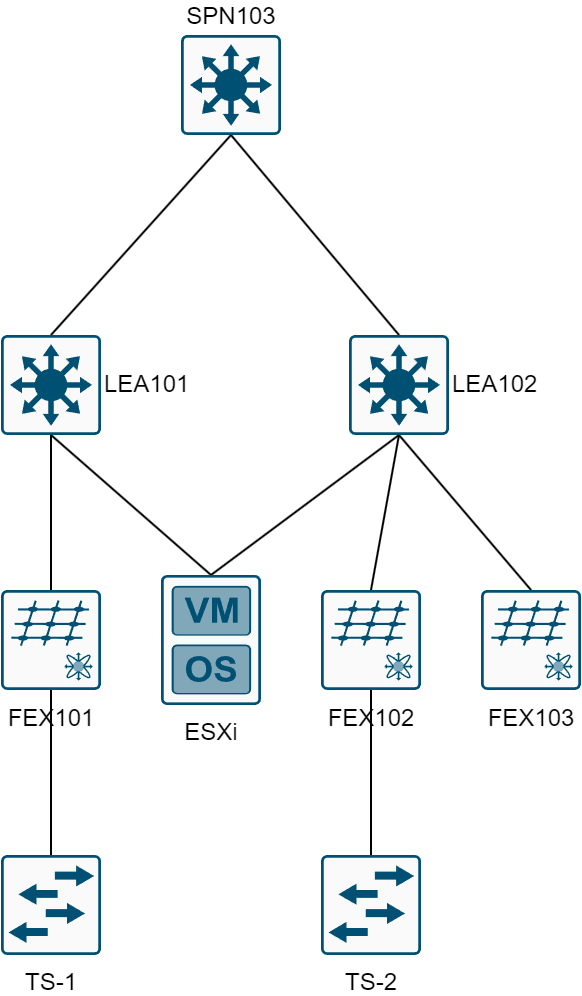
\includegraphics[width=0.5\linewidth]{images/aci-topology.png}
    \caption{Example physical deployment}
    \label{fig:example-deployment}
\end{figure}

\begin{figure}[H]
    \centering
    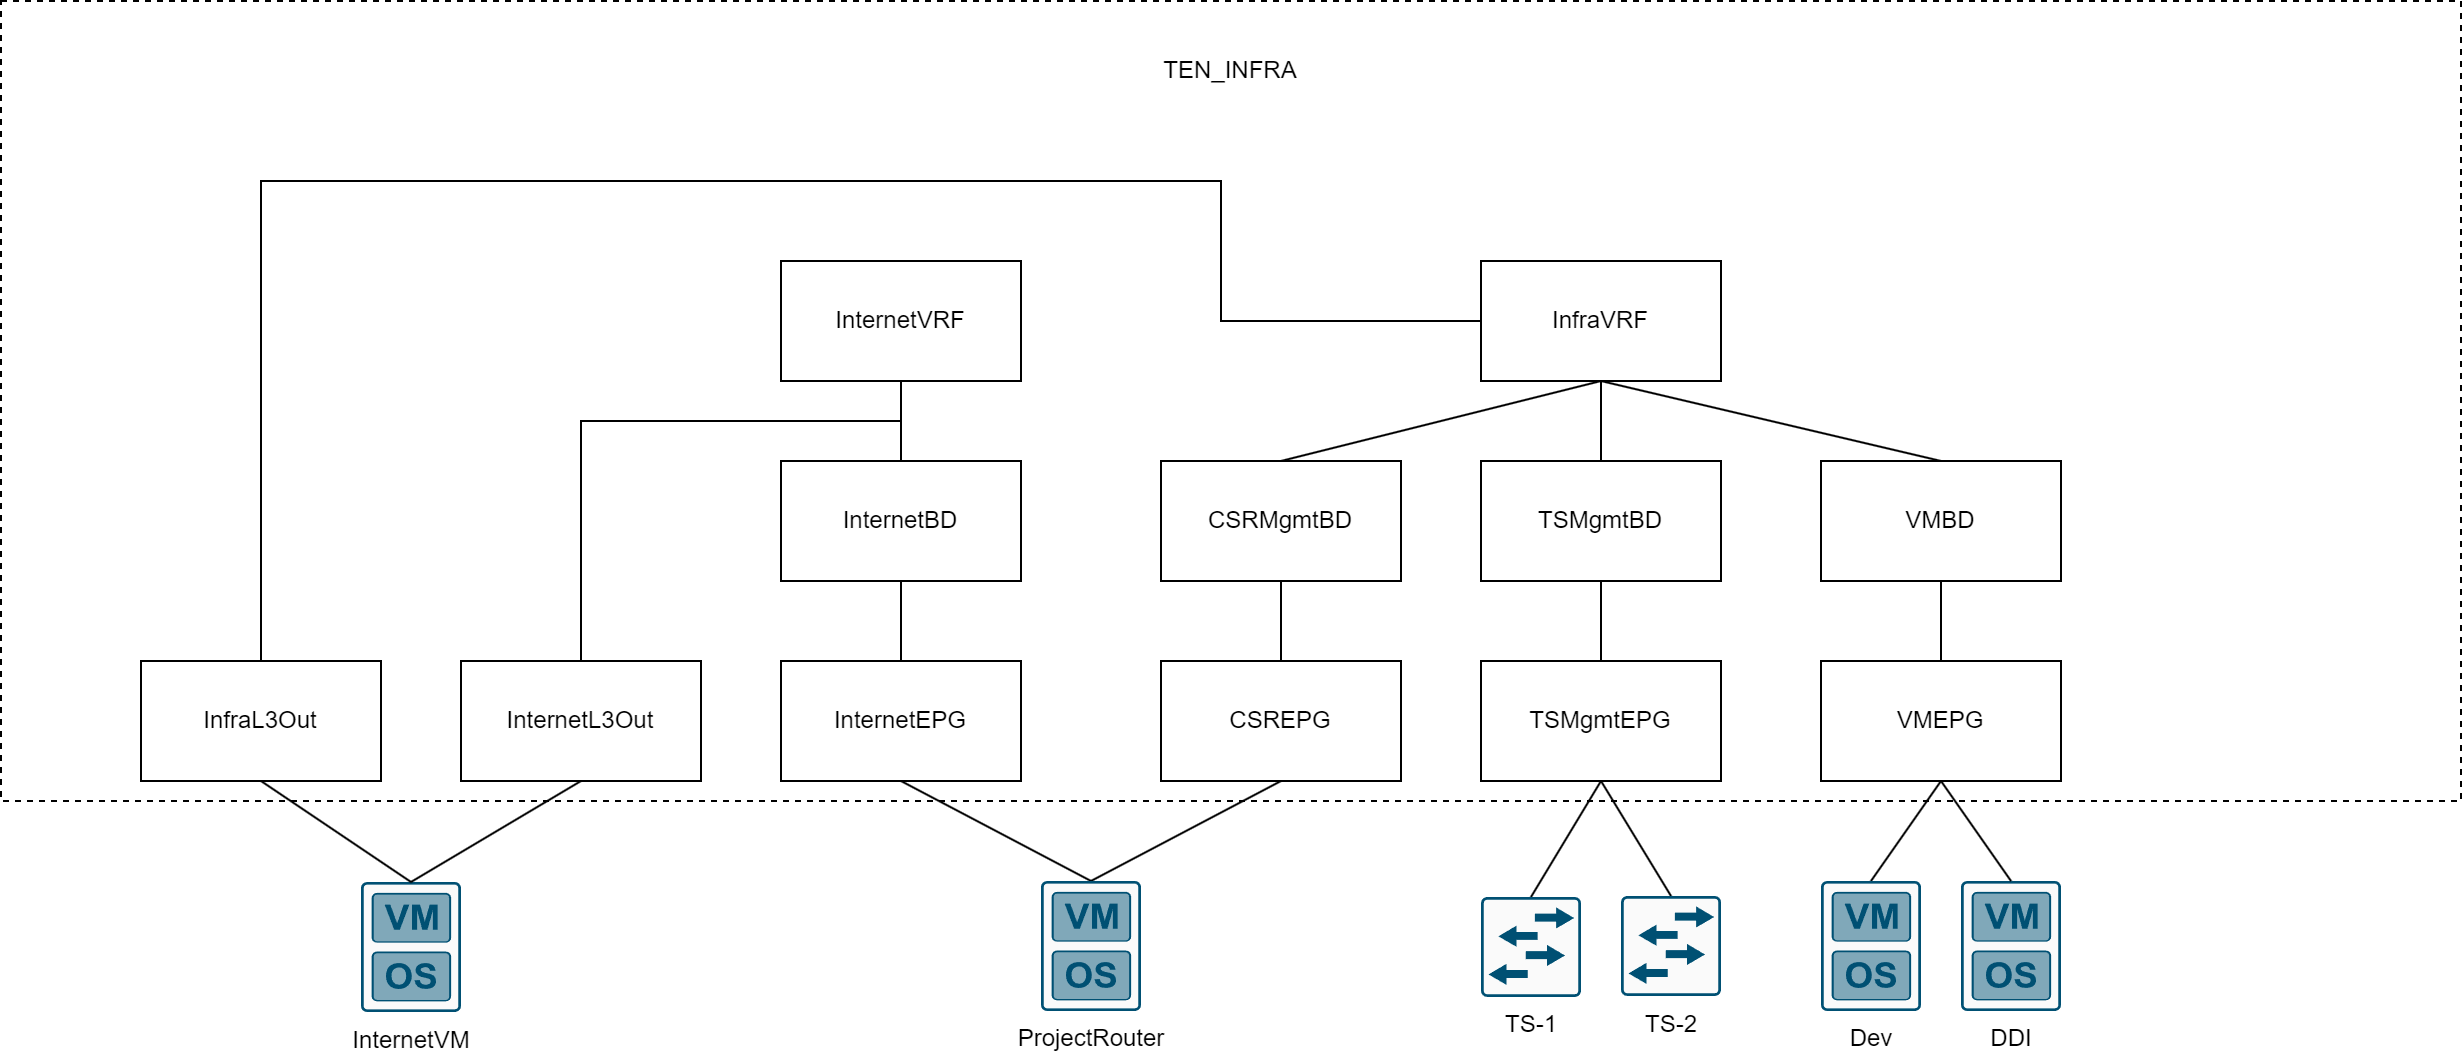
\includegraphics[width=1\linewidth]{images/epg-topology.png}
    \caption{Example ACI configuration}
    \label{fig:example-aci}
\end{figure}

\section*{ENV File Configuration}
For the automation platform to operate correctly, the .env file must be configured with the required information so that various services such as ACI and vCenter can be accessed correctly. A breakdown of the required .env file variables is provided below:
\begin{table}[H]
    \centering
    \begin{tabular}{l l p{0.4\linewidth}}
        \textbf{Variable}         & \textbf{Example} & \textbf{Description}                                                                                                \\
        \hline
        APIC\_IPADDR              & 192.168.0.125    & IP address of the APIC controller                                                                                   \\             \hline
        APIC\_USERNAME            & admin            & Username for the APIC controller                                                                                    \\            \hline
        
        APIC\_PASSWORD            & password         & Password for the APIC controller                                                                                    \\            \hline
        
        ACI\_POD                  & 1                & The pod number of the ACI fabric that the automation platform will automate                                         \\            \hline
        
        ACI\_VMWARE\_DOMAIN       & ACI-DVS          & The name of the VMM integration domain                                                                              \\            \hline
        
        ACI\_INFRA\_DOMAIN        & InfraPhys        & The name of the physical domain used to connect terminal servers to the ACI fabric                                  \\            \hline
        
        ENHANCED\_LACP            & LACP             & Name of the enhanced LACP policy used to connect ESXi nodes, leave this null if Enhanced LACP is not being utilised \\            \hline
        
        
        VSPHERE\_IPADDR           & 192.168.0.128    & IP address of the vCenter server                                                                                    \\            \hline
        
        VSPHERE\_USERNAME         & admin            & Username for the vCenter server                                                                                     \\            \hline
        
        VSPHERE\_PASSWORD         & password         & Password for the vCenter server                                                                                     \\            \hline
        
        PROJECT\_ROUTER           & ProjectRouter    & Name of the virtual router VM template                                                                              \\        \hline
        PROJECT\_ROUTER\_USERNAME & automation       & Username that will be used to connect to virtual router VM                                                          \\ \hline
        PROJECT\_ROUTER\_PASSWORD & password         & Password that will be used to connect to virtual router VM                                                          \\ \hline
    \end{tabular}
\end{table}

\section*{Virtual Router Template}
The virtual router template should be a powered-off VM, not a template, this is due to a limitation in the vCenter REST API. The VM should have the following interface assignments:
\begin{table}[H]
    \centering
    \begin{tabular}{l l l}
        \textbf{Interface} & \textbf{Port Group}                       \\
        \hline
        Network Adapter 1  & quarantine                                \\
        Network Adapter 2  & Internet EPG                              \\
        Network Adapter 3  & Virtual Router Management EPG (with DHCP) \\
    \end{tabular}
\end{table}
Network adapter 1 will automatically be assigned to the project EPG by the automation scripts. The automation script will automatically configure NAT, default route and WAN IP address, so only the 3rd network adapter needs to be configured to retrieve its IP address from DHCP. RESTCONF will also need to be enabled, sample configuration is shown below.

\begin{verbatim}
vrf definition Mgmt
 address-family ipv4
 exit-address-family
!
interface GigabitEthernet3
 vrf forwarding Mgmt
 ip address dhcp
 negotiation auto
 no mop enabled
 no mop sysid
!
ip forward-protocol nd
ip http server
ip http authentication local
ip http secure-server
ip http secure-port 1025
restconf
\end{verbatim}

Additional ACLs should be configured to secure access to RESTCONF, however, these will depend on the specific environment and deployment. Once the initial configuration is complete, the VM should be powered off and left in the desired folder where the project routers will be stored.


\section*{Solution Deployment}
In the future, the solution will be packaged via Docker Compose, which will allow one command to be run to install and serve the solution as a whole.
With ACI and vCenter configured, the automation platform can be deployed. The platform will need Docker running ideally ontop of a Linux host, however, it can be deployed on Windows using Docker Desktop. NodeJS and NPM will also be required to build and serve the front end. The following steps will need to be completed to deploy the platform:

\begin{enumerate}
    \item Clone the repository from GitHub
    \item Configure the .env file with the required information
    \item Run the following command in the back-end folder to obtain the required composer dependencies:
          \begin{verbatim}
    docker run --rm \
        -u "$(id -u):$(id -g)" \
        -v "$(pwd):/var/www/html" \
        -w /var/www/html \
        laravelsail/php82-composer:latest \
        composer install --ignore-platform-reqs
          \end{verbatim}
    \item Run the following command in the back-end folder to start the platform:
          \begin{verbatim}
    ./vendor/bin/sail up -d
    ./vendor/bin/sail artisan key:generate
    ./vendor/bin/sail artisan migrate
    ./vendor/bin/sail artisan queue:listen --timeout 400
            \end{verbatim}
    \item Run the following command in the front-end folder to obtain the required node dependencies:
    \begin{verbatim}
    npm install
    npm run build
    npm run start
    \end{verbatim}
\end{enumerate}

When first connecting to the solution, navigate to the ACI page and select the VLAN pool that was created in ACI for use by the automation platform. Then click Set Interface Profiles, and assign the corresponding interface profile to each node discovered by the automation platform. Once this is complete, the solution is ready to be used. Figure \ref{d:interface-assignment} shows an example mapping:

\begin{figure}[H]
    \centering
    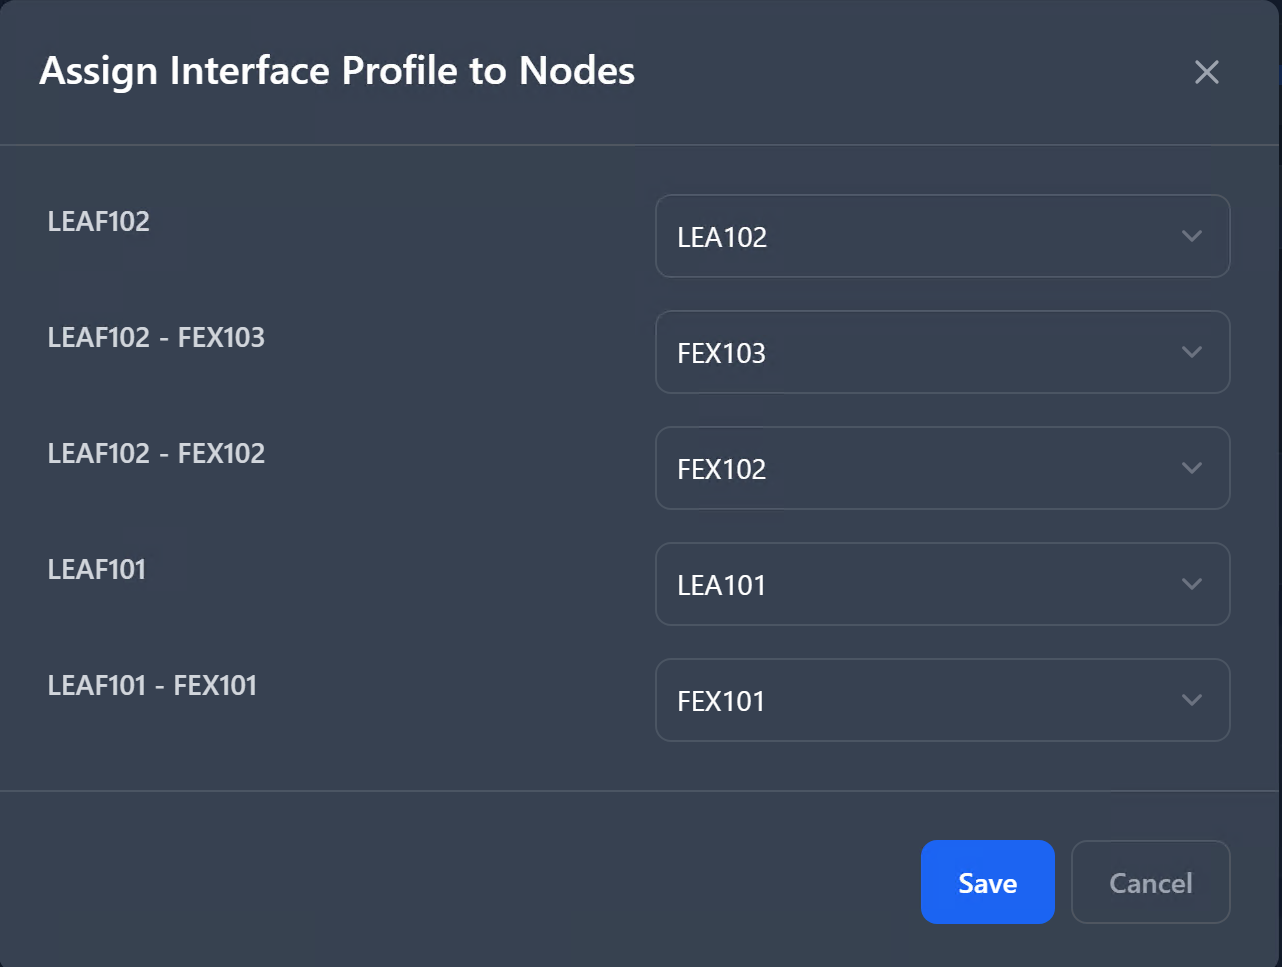
\includegraphics[width=0.6\linewidth]{images/interfaceprof-mapping.png}
    \caption{Example interface profile assignment}
    \label{d:interface-assignment}
\end{figure}

Terminal servers should also be added via the terminal servers page, where all information the platform needs is required on the addition form.